\section{Implementation audit and reproducible observations}
\label{sec:validation}

The mathematical statements above concern exact operations on specified
inputs. The experiments in this section check their relationship to the
delivered implementation. They also measure costs on complete public
queries, where source reconstruction, unchanged operations, and output
serialization can dominate the improved subroutine. The retained raw
records are the basis of every numerical table; the plotting script reads
those records directly.

\subsection{The changed trust boundary}

The old public weighted checker authenticates the source pairings and
weight intervals, verifies the unweighted AHT trace, reconstructs the
initial weight function, evaluates its transport, compares the final
histogram, and checks conservation. The new checker retains all these
steps and the same certificate schema. It changes the transport callback
to a local run-tree implementation.

The original flat transport remains executable as
\code{verify_weighted_orbit_certificate_reference}. The producer remains
separately implemented and does not import the new run tree. In particular,
the producer's quotient/remainder transport and the checker's
residue-anchor derivative are different arithmetic constructions of the
same push-forward. The separate weighted least-representative checker
also retains its earlier transport. Its forward weights and reverse
representative recovery are not silently replaced by histogram replay.

The chamber exporter introduces a new observer and certificate schema.
Its checker reconstructs marker addresses and chamber identifications
through the independent raw cut-cell reference described in
Section~\ref{sec:chambers}. Independence here means separate source
reconstruction and arithmetic paths at the stated interfaces. Both
checkers still rely on the established source validators, integer codec,
and unweighted orbit verifier. This is not a claim that every underlying
primitive has been independently reimplemented.

\subsection{Focused differential and adversarial tests}

The replay change passed 52 focused native test methods in a recorded
124.207-second run. These include the maintained moment-boundary test's
entire 157-source bank and full supplied-cut handlebody replay with
production paths disabled. Seven new test methods include:

\begin{itemize}
\item 500 random lazy range-add, split, and join transitions, checking the
full AVL height invariant, subtree lengths, endpoint values, and canonical
run sequence after every transition;
\item 1,000 random signed-vector translation folds, and every admitted
reflection fold, compared with literal point-fibre sums;
\item 400 random static deletions, with exact deleted histograms and the
remaining function compared with a literal reference;
\item interval lengths requiring more than 8,192 bits, without literal
expansion of the interval;
\item complete native star-family proofs accepted through both public
verifier variants, malformed-proof rejection, conservation checks, and
propagation of callback cancellation.
\end{itemize}

The eleven new chamber test methods independently exercise source labels,
two-sidedness, side markers, graph reconstruction, and subcuts. They include
nonzero triangle and quadrilateral ranks, signed edge identifications,
vertex and tetrahedron relabellings, representative reorderings, and an
actual reversal of the local coorientation. Multiple representatives on
one component are tested using distinct discs as invalid component labels.
Other cases cover omitted components, one-sided surfaces and their
connected two-sided doubles, empty surfaces, source and proof mutations,
hexadecimal integer encodings, booleans in integer fields, disabled
producers, shared work limits, and callback cancellation.

The maintained native suite was then run after the source files stabilized.
The broad run executed 1,733 methods in 499.532 seconds, with two failed
assertions and one class-setup error caused by a missing external fixture.
After restoring the exact pinned fixture, all eight methods in that class
passed. Thus the completed audit exercised all 1,741 declared methods.
The exact logs are \code{results/full_native_suite.log} and
\code{results/transport_annulus_fixture_rerun.log}.

Both failed assertions were independently reproduced in fresh workers using
the exact pinned source and in workers using the lazy patch: each expected
\code{INCONCLUSIVE} but received \code{COMPLETE}. They occur in
\code{test_core_primitive_annuli.py} and
\code{test_disk_bundle_absorption.py}; the pinned adaptive lower-forest
tests explicitly require the successful outcomes on those same sources.
The source-authenticated baseline audit retains the identical tracebacks
and hashes in \code{results/baseline_failure_audit.json}. These two stale
expectations remain unchanged. No additional source failure was observed.

An earlier verbose attempt was interrupted during a filesystem-capacity
incident; its partial log is retained separately and is not counted as
completed regression evidence. The restored-fixture run described above
resolves the environmental setup error. These are executed finite
regression and differential checks, not a proof-assistant formalization
of the article's theorems.

\subsection{Complete weighted-certificate measurements}

Table~\ref{tab:star-timing} measures the entire public weighted-certificate
verification call for the star family. It includes source weight
validation, initial canonicalization, independent authentication of the
unweighted trace, and final histogram checks. Certificate generation is
recorded separately and is outside this timed interval.
Each row contains three paired repetitions. The figure shows all samples
and the median for each backend.

\begin{table}[htbp]
\centering\small
\begin{tabular}{rrrrr}
\toprule
$H$ & $L$ & Flat (s) & Lazy (s) & Ratio \\
\midrule
16 & 256 & 0.008291 & 0.002036 & 4.073$\times$ \\
32 & 1,024 & 0.075450 & 0.007252 & 10.404$\times$ \\
64 & 4,096 & 0.602308 & 0.030957 & 19.456$\times$ \\
128 & 16,384 & 4.745231 & 0.121760 & 38.972$\times$ \\
\bottomrule
\end{tabular}

\caption{Median complete weighted verification times on the legal star
family. A ratio greater than one means the lazy variant was faster.
Here \(L=H^2\); all displayed widths are even.}
\label{tab:star-timing}
\end{table}

\begin{figure}[htbp]
\centering
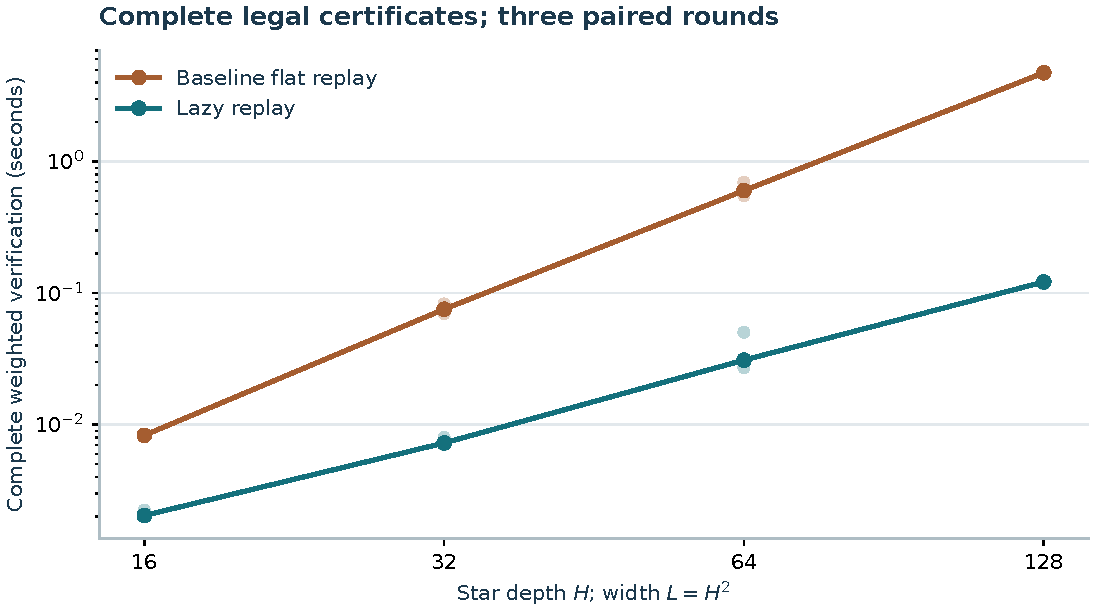
\includegraphics[width=0.93\textwidth]{figures/synthetic_replay.pdf}
\caption{Observed complete weighted replay on one machine. The pale
points are the three individual measurements; connected points are
medians. The proof of Theorem~\ref{thm:star}, rather than a fitted timing
curve, establishes the asymptotic separation.}
\label{fig:star-timing}
\end{figure}

At \(H=128\), the initial state has 16,384 runs. The complete native trace
contains 128 truncations and one contraction. The instrumentation records
128 removed suffix runs in total, 255 range additions, and 16,384 emitted
runs. Reading a receiving subtree's stored run count records over two
million receiver-run incidences without visiting those leaves. The final
histogram has precisely two entries, weights 128 and 129, each with
multiplicity 8,192. These counters connect the measured example to the
mechanism in the proof.

The implementation was measured under Python 3.12.14 on a Linux x86-64
environment. The full interpreter and platform strings are stored with
the data. Three repetitions on one shared host do not establish a
hardware-independent speed factor or a statistical confidence interval.
The source family demonstrates a legal orbit-trace obstruction to eager
replay; no claim is made that these orbit systems are a family of hard
knot-complement normal cuts.

\subsection{Paired native supplied-cut queries}

The native benchmark uses eleven source/method pairs: eight maintained
case/method choices and three genuine layered-solid-torus meridians with
coordinates multiplied by three. It includes both moment and mask boundary
methods. Raw triangulations and coordinates are bundled, so replay needs
no fixture generator or Regina installation.

The old and new verifiers run in isolated Python processes. The baseline
package is restored using the exact pinned verifier bytes; no module-binding
monkeypatch substitutes an old implementation at runtime. In each of three
paired rounds, the benchmark freshly reconstructs the source, produces a
complete supplied-cut certificate, runs public whole-cut verification, and
serializes the result as canonical JSON. Every certificate was independently
accepted and every complete-result digest agreed between the variants.
Source preparation is included in the relevant production and verification
calls, rather than reported as an omitted preprocessing step.

\begin{table}[htbp]
\centering\footnotesize
\setlength{\tabcolsep}{4pt}
\begin{tabular}{lrrrr}
\toprule
Source/method & Flat replay & Lazy replay & Replay ratio & Query ratio \\
\midrule
Pilot LST, moments & 0.0141 & 0.0139 & 1.011 & 1.004 \\
Pilot trefoil, moments & 0.0038 & 0.0038 & 0.992 & 1.004 \\
Solid torus/RP3, moments & 0.0119 & 0.0126 & 0.942 & 0.948 \\
Interior mixed, moments & 0.0656 & 0.0483 & 1.360 & 1.169 \\
Fibonacci 09 mixed, moments & 0.7988 & 0.5812 & 1.374 & 1.134 \\
Trefoil mixed, moments & 0.1302 & 0.1109 & 1.174 & 1.111 \\
Pilot LST, masks & 0.0178 & 0.0150 & 1.186 & 1.123 \\
Interior mixed, masks & 0.0618 & 0.0517 & 1.195 & 1.271 \\
Layered meridian $T=4$ & 0.2043 & 0.1510 & 1.353 & 1.122 \\
Layered meridian $T=8$ & 0.8797 & 0.7274 & 1.209 & 1.087 \\
Layered meridian $T=16$ & 3.9349 & 3.4831 & 1.130 & 0.925 \\
\midrule
Sum of case medians & 6.1229 & 5.1989 & 1.178 & 0.982 \\
\bottomrule
\end{tabular}

\caption{All native paired results. Replay times are seconds; ratios
are baseline/new medians. The query ratio includes production, whole-cut
verification, and serialization. The layered rows use moments and scale
three. The final row is a ratio of sums of case medians.}
\label{tab:native-timing}
\end{table}

The sum of case-median replay times decreased from 6.122913 to 5.198893
seconds, a ratio of \(1.1777\). The corresponding complete-query totals
were 14.109865 and 14.364058 seconds: the new run was approximately
\emph{1.8 percent slower}. The data therefore support an aggregate replay
improvement but do not support an aggregate complete-query speed-up.

The largest discrepancy occurred in the \(T=16\) layered case. Its unchanged
producer took median 5.253965 seconds in the baseline worker and 6.811022
seconds in the new worker, while whole-cut verification improved from
3.934936 to 3.483064 seconds. The producer source is identical between
variants. These measurements alone do not establish the cause of its
time variation. The original samples, including the unfavorable aggregate
and the small-case regression, are retained without replacement.

The timing scope is a supplied normal-cut handlebody census, not a
diagram-to-verdict unknot run. It is also broader than the changed ordinary
weighted replay: two representative-selector queries and other source
work remain unchanged. These facts explain why the synthetic verifier
ratios cannot be multiplied into a claimed recognition speed factor.
A controlled repetition addressing the producer variation is a useful
future experiment; it is not a reason to discard the present observation.

\subsection{Geometric chamber checks on native inputs}

The maintained corpus contains 106 inputs. Among 99 inputs small enough
for the deliberately bounded literal reference, 80 produced independently
accepted chamber graphs and 19 were correctly refused because their
surfaces contain a one-sided component. The seven remaining binary
multiplicity cases correctly refused an incomplete representative list.
An inconclusive response on those inputs is a source-contract outcome,
not a negative topological verdict.

For all accepted small inputs, 254 exhaustive labelled subbatch checks
agreed with \emph{two} independent literal constructions. The first
reglues every actual normal-disc face of each omitted component into the
full cut. The second forms the normal vector of exactly the selected
components, independently regenerates that subcut, and counts its
literal chamber components. The components themselves are identified by
gluing individual face-arc disc ranks, rather than by reusing the native
normal-edge orbit census. These checks cover separating bridges,
one-vertex loops, mixed systems, and the three-cycle in
Figure~\ref{fig:three-meridians}.

Large-coordinate connected meridians were checked separately.
Table~\ref{tab:chamber-stress} records single feasibility samples, without
a baseline or comparative speed claim.

\begin{table}[htbp]
\centering\small
\setlength{\tabcolsep}{4pt}
\begin{tabular}{rrrrrr}
\toprule
$T$ & Coordinate bits & Orbit cycles & Proof bytes & Produce (s) & Replay (s) \\
\midrule
16 & 11 & 110 & 147,835 & 0.0167 & 0.0125 \\
32 & 22 & 206 & 555,642 & 0.0613 & 0.0311 \\
64 & 44 & 398 & 2,165,507 & 0.2722 & 0.0991 \\
128 & 89 & 782 & 8,538,169 & 1.1494 & 0.3594 \\
\bottomrule
\end{tabular}

\caption{Connected meridians of Fibonacci layered solid tori.
Proof size is compact uncompressed JSON bytes. Each graph consists of
one vertex and one loop.}
\label{tab:chamber-stress}
\end{table}

The \(128\)-tetrahedron example has exactly
\[
2\,791\,715\,456\,571\,051\,233\,611\,642\,548
\]
normal discs, maximum coordinate bit length 89, and one component. A
representative at a large nonzero quadrilateral rank authenticates its
one-loop graph. The certificate has 8,538,169 bytes and the three queries
use 782 orbit cycles. The corresponding single observed production and
replay times were 1.149 and 0.359 seconds.

These connected examples use the maintained single-orbit shortcut in the
weighted queries. They demonstrate that native graph authentication can
handle enormous literal disc counts at small component count; they are
not a separate benchmark of the new lazy fold. The complete small
three-meridian packet and the \(128\)-tetrahedron packet are retained so
that their source validation and graph replay can be repeated directly.
